\documentclass[12pt]{article}
\pagestyle{headings}
\setlength{\textheight}{8.67in}
\setlength{\textwidth}{5.8in}
\setlength{\topmargin}{-3mm}
\setlength{\headsep}{40pt}
\setlength{\evensidemargin}{-3mm}
\setlength{\parskip}{.05in}
\setlength{\parindent}{3ex}
\renewcommand{\baselinestretch}{1.2}
\usepackage{amsthm}
\usepackage{graphicx}
\setlength{\headsep}{40pt}
\usepackage{graphicx}
\usepackage{color}
\usepackage{array}
\usepackage{amsmath,amssymb}
\usepackage{epstopdf}
\usepackage{tikz}
\setlength{\topmargin}{-3mm}
\setlength{\leftmargin}{.1in}
\setlength{\footskip}{0.5in}
\pagestyle{myheadings}
\pagenumbering{arabic}
\theoremstyle{definition}
\setlength{\unitlength}{1cm}
\thicklines
\newtheorem{ex}{Example}
\begin{document}
	\title{\textbf{Linear Transformation on Linear Space} \\
		\large\underline{Internship Report} 
	}
	\author{Anshada P.M}
	\date{July,2019}
	\maketitle
	\pagenumbering{arabic}
	\section{Linear Transformation}
	Let $ V $ and $W $ be an n dimensional vector space over a field $ \mathbb{F} $. Let $ T :V\rightarrow W $ be a function with $ V $ as its domain and its range contained in $ W $. $$ T(V)\subset W $$$ T $ is linear in the sense that $$ T(v_1 + v_2) = T(v_1)+T(v_2) $$ $$ T(\alpha v_1)=\alpha T(v_1)$$ 
	$\forall$ $ v_1,v_2 \in V$ and $\alpha\in\mathbb{F}$.\\
	
	\begin{picture}(10,3)
	\put(3,2){\circle{4}}
	\put(2.8,2.8){V}
	\put(8,2){\circle{4}}
	\put(7.8,2.8){W}
	\qbezier(3,2)(5.5,4)(7.8,2)
	\put(5.5,2.995){\vector(1,0){0.2}}
	\put(5.5,2.5){$ T $}
	\put(2.7,2){$ v $}
	\put(7.9,2){$ T v $}
	\end{picture}
	\\
	Let $ L(V,W) $ denote the set of linear transformation from $V$ to $W.$ If $ T\in L(V,W),$ $T$ is defined if we prescribe the action of T on a basis of $V$.\\
	\\
	Let $\mathcal{B} = {v_1,v_2,...,v_n}$ be a basis of V.
	Then $v\in V$ given by $v = x_1v_1+x_2v_2+...+x_nv_n$ , $\forall$ $x_i$ $\in \mathbb{F}$
	$$T(v) = T(x_1v_1+x_2v_2+...+x_nv_n)$$
	$= x_1T(v_1)+x_2T(v_2)+...+x_nT(v_n)$\\
	If we know every $T(v_i)$ we will get T(v).\\              
	Let $ T $ be the linear transformation from $ \mathbb{P}_{2}(\mathbb{R}) $ to $ \mathbb{R}^{3} $ defined by $ \phi(p):= $ ($ p_{0} $ $ p_{1} $ $ p_{2} $). Let $ \mathfrak{B}_{1}=\{1,t,t^2\} $ be the basis for the vector space $ \mathbb{P}_{2}(\mathbb{R}) $. So the function can be represented as $p_{0}+p_{1}t+p_{3}t^2\to  $($ p_{0} $ , $ p_{1} $ , $ p_{2} $).  $$ T_{\mathfrak{B}_{1}}=\phi $$
	Let $ \mathfrak{B}_{2}=\{1+t,1-t,t+t^2\} $ be another basis in $ \mathbb{P}_{2}(\mathbb{R}) $. Then $$ p=q_{0}(1+t)+q_{1}(1-t)+q_{2}(t+t^2) $$
	$ \hspace*{4.4cm}=(q_{0}+q_{1})+(q_{0}-q_{1}+q_{2})t+(q_{2}t^2) $$$ \implies  q_{0}+q_{1}=p_{0},q_{0}-q_{1}+q_{2}=p_{1} ,q_{2}=p_{2}$$$$ q_{0}=\frac{1}{2}(p_{0}+p_{1}-p_{2}),q_{1}=\frac{1}{2}(p_{0}+p_{1}+p_{2}) ,q_{2}=p_{2}$$\\The transformation with respect to the basis $ \mathfrak{B}_{2} $ can be represented as  $$ T_{\mathfrak{B}_{2}}=\psi(p)=(q_{0},q_{1},q_{2}) $$$ \hspace*{6.1cm}= $($ \frac{1}{2}(p_{0}+p_{1}-p_{2}) $ , $ \frac{1}{2}(p_{0}1p_{1}+p_{2})  $ , $ p_{2} $)
	\begin{center}		
		
		\begin{picture}(8,5)
		\put(2,3.2){\circle{2.5}}
		\put(1.5,4){$ \mathbb{F}^n $}
		\put(6,3.2){\circle{2.5}}
		\put(6,4){$ \mathbb{F}^n $}
		\put(4,0.2){\circle{2.5}}
		\put(2.2,0){$ \mathbb{P}_2(\mathbb{R}) $}
		\put(1.3,3.2){$\phi(u)$}
		\put(5.7,3.4){$\psi(u)$}
		\put(4.,-0.1){$u$}
		\qbezier(2,3.2)(4,4)(6,3.2)
		\put(4,3.6){\vector(1,0){0.2}}
		\put(3.8,3.9){$ \psi\phi^{-1} $}
		\qbezier(4,0.2)(4,2)(6,3.2)
		\put(4.3,1.6){\vector(1,1){0.2}}
		\put(4.5,1.6){$ \psi $}
		\qbezier(4,0.2)(2,2)(2,3.2)
		\put(2.6,1.7){\vector(-1,1){0.1}}
		\put(2.2,1.6){$ \phi $}
		%\put(4,1.2){\oval(4,2)[r]}
		\end{picture}
	\end{center}
	\section{Matrix Representation of Linear Transformation}
	 Let $U$ be an n-dimensional vector space over the field $ \mathbb{F}$ and $V$ an m-dimensional vector space over $\mathbb{F}$. Let $\mathcal{B}$:=$\{u_1,u_2,...,u_n\}$ be an ordered basis for $U$ and $\mathcal{B\prime}$:=$\{v_1,v_2,...,v_m\}$ an ordered basis for $V$. For each linear transformation $T$ from $U$ into $V$, there is an $ m\times n$ matrix $\mathbf{A}$ with entries in $\mathbb{F}$.\\
	 Let $T$ be given by
 	 $$ T(u_{i})=a_{1_{i}}v_1+a_{2_{i}}v_2+...+a_{m_{i}}v_m $$
	  i = (1,2,...,n)\\
	  Let $u\in U$, then $u = x_1u_1+x_2u_2+...+x_nu_n$\\
	  $T(u) = x_1T(u_1)+x_2T(u_2)+...+x_nT(u_n)$\\
	  \hspace*{1cm}= $x_1(a_{1_{1}}v_1+...+a_{1_{n}}v_m	)+...+x_n(a_{m_{1}}v_1+...+a_{m_{n}}v_m	)$
	  The matrix representation of $T$,that is $\mathbf{A}$ is given by $a_{i_{j}}.$\\
	  $
	  \mathbf{A} =
	  \begin{bmatrix}
	  a_{1_{1}} & a_{1_{2}} & ... &a_{1_{n}}\\
	  a_{2_{1}} & a_{2_{2}} & ... &a_{2_{n}}\\
	  ...&...&...&...\\
	  a_{m_{1}} & a_{m_{2}} & ... &a_{m_{n}}\\
	  \end{bmatrix}
	  $
	  ,an $m\times n$ matrix.
	  
	  \begin{center}
	  	\begin{picture}(7,7)
	  	%\put(0,0){0,0}\put(8,0){8,0}\put(0,8){0,8}\put(8,8){8,8}
	  	\put(2,2){\circle{4}}\put(6,2){\circle{4}}\put(2,6){\circle{4}}\put(6,6){\circle{4}}
	  	\qbezier(2,6)(4,7)(6,6)\put(4,6.5){\vector(1,0){0.2}}
	  	\qbezier(2,2)(4,1.4)(6,2)\put(4,1.689){\vector(1,0){0.2}}
	  	\qbezier(2,6)(1,4)(2,2)\put(1.5,4){\vector(0,1){0.2}}
	  	\qbezier(6,6)(5,4)(6,2)\put(5.5,4){\vector(0,1){0.2}}
	  	\put(4,6.7){$ \mathbf{A} $}\put(0.9,4){$ {\phi}_\mathcal{B} $}\put(4.7,4){$ {\phi}_\mathcal{B\prime} $}\put(4,1.3){$ T$}
	  	\put(1.6,1.8){$ u $}\put(2.1,2.1){$ \mathbb{U} $}
	  	\put(5.8,1.6){$Tu $}\put(6.1,2.1){$ \mathbb{V} $}
	  	\put(-0.15,5.9){
	  		$ 
	  		\begin{pmatrix} 
	  		x_1\\
	  		x_2\\
	  		...\\
	  		x_n
	  		\end{pmatrix}=x
	  		$}
  		\put(1.9,6.3){$ \mathbb{F}^{n} $}
	  	\put(6,5.9){
	  		$
	  		y =
	  		\begin{pmatrix} 
	  		y_1\\
	  		y_2\\
	  		...\\
	  		y_m
	  		\end{pmatrix}
	  		$}
  		\put(5.65,6.3){$ \mathbb{F}^{m} $}
	  	\end{picture}
	    \end{center}
      Let $u\in U$ and $T(u)=v$,where $v\in V.$\\
  	  Let ${\phi}_\mathcal{B}(u)=x, x\in\mathbb{F}^{n}$,\\
  	  \hspace*{0.6cm}	${\phi}_\mathcal{B\prime}(v)=y, y\in\mathbb{F}^{n}$\\
  	  $\implies {\phi}_\mathcal{B\prime}(Tu)=y$\\
  	  $\implies {\phi}_\mathcal{B\prime}\circ T(u)=y$\\
  	  $\implies {\phi}_\mathcal{B\prime}\circ T({{\phi}_\mathcal{B}}^{-1}x)=y$ ,  ${\phi}_\mathcal{B}u = x$\\
  	  $\implies {\phi}_\mathcal{B\prime}\circ T\circ{{\phi}_\mathcal{B}}^{-1}(x)=y $\\
  	  Since $\mathbf{A}x = y$, we will get 
  	  $\boxed{\mathbf{A} =  {\phi}_\mathcal{B\prime}\circ T\circ{{\phi}_\mathcal{B}}^{-1}}$-
	  \section{Similarity Transformation}
	  Let $V$ be an n dimenstional vector space. $T$ is a linear transformation such that $T \in L(V) $.Let $\mathcal{B}$:=$\{v_1,v_2,...,v_n\}$ and $\mathcal{B\prime}$:=$\{v\prime_1,v\prime_2,...,v\prime_m\}$ be an ordered basis for $V$.\\ $\phi$ is a function under basis $\mathcal{B}$, $\phi={\phi}_\mathcal{B}$.\\$\psi$ is a function under basis $\mathcal{B\prime}$, $\psi={\psi}_\mathcal{B\prime}$.
	  \begin{center}
	  	\begin{picture}(8,10)
	  	%\put(0,0){0,0}\put(8,0){8,0}\put(0,10){0,10}\put(8,10){8,10}
	  	\put(2,1){\circle{4}}\put(2,5){\circle{4}}\put(2,9){\circle{4}}\put(6,1){\circle{4}}\put(6,5){\circle{4}}\put(6,9){\circle{4}}
	  	\qbezier(2,1)(4,2)(6,1)\put(4,1.5){\vector(1,0){0.2}}\put(3.7,1.7){$[T]_{\psi}= \mathbf{A}$}\qbezier(2,5)(4,6)(6,5)\put(4,5.5){\vector(1,0){0.2}}\put(3.9,5.7){$T$}\qbezier(2,9)(4,10)(6,9)\put(4,9.48){\vector(1,0){0.2}}\put(3.7,9.7){$ [T]_{\phi} = \mathbf{B} $}
	  	\qbezier(2,1)(1.5,3)(2,5)\put(1.75,3){\vector(0,-1){0.2}}\put(1.85,2.85){$\psi$}\qbezier(6,1)(5.5,3)(6,5)\put(5.75,3){\vector(0,-1){0.2}}\put(5.85,2.85){$\psi$}\qbezier(2,9)(1.5,7)(2,5)\put(1.75,7){\vector(0,1){0.2}}\put(1.85,7){$\phi$}\qbezier(6,9)(5.5,7)(6,5)\put(5.75,7){\vector(0,1){0.2}}\put(5.85,7){$\phi$}\qbezier(2,9)(-1,5)(2,1)\put(0.5,5){\vector(0,-1){0.2}}\put(-1.5,4.85){$\psi\phi^{-1}=\mathbf{C}$}\qbezier(6,9)(9.,5)(6,1)\put(7.5,5){\vector(0,-1){0.2}}\put(7.67,4.85){$\psi\phi^{-1}=\mathbf{C}$}
	  	\put(1.7,0.6){$\mathbb{F}^{n}$}\put(5.8,0.6){$\mathbb{F}^{n}$}\put(1.7,9.1){$\mathbb{F}^{n}$}\put(6,9.1){$\mathbb{F}^{n}$}\put(6.1,4.9){$\mathbb{V}$}\put(1.6,4.9){$\mathbb{V}$}
	  	\end{picture}
	  \end{center}
  	  $${[T]}_\phi = \phi{\psi}^{-1}{[T]}_\psi({\phi{\psi}^{-1}})^{-1}$$
  	  $\implies$ $$\mathbf{B}={\mathbf{C}}^{-1}\mathbf{A}\mathbf{C}$$
  	  where C is an invertible $n\times n$ matrix, and $\mathbf{C} = \phi{\psi}^{-1}$\\
	  If $\mathbf{A}$ and $\mathbf{B}$ be n$\times$n (square) matrices over field $\mathbb{F}$. We say that $\mathbf{B}$ is similar to $\mathbf{A}$ over $\mathbb{F}$, if there is an invertible n$\times$ n matrix $\mathbf{C}$ over $\mathbb{F}$ such that  $\mathbf{B}$=$\mathbf{C^{-1}}\mathbf{A}\mathbf{C}$.There exist an equivalence relation between the matrices like $\mathbf{A}$ and $\mathbf{B}$.\\
	  $\mathit{ Proof}:$ Let $\mathbf{X},\mathbf{Y},\mathbf{Z}\in \mathbf{M}_{n\times n}(\mathbb{R})$,\\
	  $\forall$ $\mathbf{X}\in \mathbf{M}_{n\times n}(\mathbb{R})$ , $\mathbf{X}={\mathbf{I}}^{-1}\mathbf{X}\mathbf{I}$ \\
	  So,$\mathbf{X} \sim \mathbf{X}, $(Reflexive relation)\\
	  Let $\mathbf{X} \sim \mathbf{Y}$, then $\mathbf{X}={\mathbf{C}}^{-1}\mathbf{Y}\mathbf{C}$\\
	  $\implies \mathbf{Y}=\mathbf{C}\mathbf{X}{\mathbf{C}}^{-1}$, so $\mathbf{Y} \sim \mathbf{X}$ ,(Symmetric relation)\\
	  Let $\mathbf{X} \sim \mathbf{Y}, \mathbf{Y} \sim \mathbf{X}$ then,\\
	  $\mathbf{X}={\mathbf{C}}^{-1}\mathbf{Y}\mathbf{C}$\\
	  $\mathbf{Y}={\mathbf{D}}^{-1}\mathbf{Z}\mathbf{D}$,\\ $\mathbf{C}$ and $\mathbf{D}$ are invertible matrix. \\
	  $\implies $ $\mathbf{X}={\mathbf{C}}^{-1}{\mathbf{D}}^{-1}\mathbf{Z}\mathbf{D}\mathbf{C}$\\
	  $\hspace*{1.4cm}=({\mathbf{D}\mathbf{C}})^{-1}\mathbf{Z}\mathbf{D}\mathbf{C}$\\
	  $\implies \mathbf{X}\sim\mathbf{Z}$(Transitive Relation)\\
	  Thus $\mathbf{B}$=$\mathbf{C^{-1}}\mathbf{A}\mathbf{C}$ an equivalence relation.\\
	  This relation $\sim$ induces a partition within the matrices also.\\
	  \begin{center}
	  	\begin{tikzpicture}
	  	\draw (2,2) circle (2cm);
	  	%\draw[step=1cm,gray,very thin] (0,0) grid (4,4);
	  	\qbezier(0,2)(2,2.5)(2,0)\qbezier(1,2)(2,3)(1,3.7)
	  	\qbezier(1.5,3)(2,2.5)(3.7,3)\qbezier(3.8,1)(3,2)(1.9,1)
	  	\put(2,2){$ M^{nxn}(\mathbb{F}) $}
	  	\end{tikzpicture}
	  \end{center}
	  Equivalent matrix represents the same linear transformation. The matrices which are not in the same partition cannot involve in the same linear transformation.\\
	  \\
	  $\mathbf{Example:}$Zero matrix is the only element in its partition.
	  \section{Diagonal Matrix}
	  Does there exist a 'simple' matrix with as many zero entries representing a given linear transformation?\\
	  A simple non-trivial matrix will be diagonal matrix.\\
	  Let $ T:V\to V $ and $ \mathfrak{B} =\{u_{1},u_{2},...,u_{n}\} $ be the basis for the set V.\\
	  If $f(t)$ is a polinomial in $\mathbb{F}$ and $T$ is represented by a diagonal matrix . 
	  $
	  \Lambda =
	  \begin{bmatrix}
	  \lambda_{1} & 0 &... & 0 \\
	  0 & \lambda_2 & ... & 0 \\
	  0 & 0 & ... & 0 \\
	  0 & 0 & ... &  \lambda_n  \\
	  \end{bmatrix}
	  $
	  \\
	  then $P(T)$ is presented with respect to the same basis by 
	  $
	  P_{\lambda}
	  \begin{bmatrix}
	  P_{\lambda_{1}} & 0 &... & 0 \\
	  0 & P_{\lambda_2} & ... & 0 \\
	  0 & 0 & ... & 0 \\
	  0 & 0 & ... &  P_{\lambda_n}  \\
	  \end{bmatrix}
	  $
	  When $T \in L(V)$, does there exist an ordered basis for $V$ with respect to $T$ so that $T$ has a diagonal representation?If such a diagonal representation exists,how to find the ordered basis?\\
	  \begin{center}
	  	\begin{picture}(7,7)
	  	%\put(0,0){0,0}\put(8,0){8,0}\put(0,8){0,8}\put(8,8){8,8}
	  	\put(2,2){\circle{4}}\put(6,2){\circle{4}}\put(2,6){\circle{4}}\put(6,6){\circle{4}}
	  	\qbezier(2,6)(4,7)(6,6)\put(4,6.5){\vector(1,0){0.2}}
	  	\qbezier(2,2)(4,1.4)(6,2)\put(4,1.689){\vector(1,0){0.2}}
	  	\qbezier(2,6)(1,4)(2,2)\put(1.5,4){\vector(0,1){0.2}}
	  	\qbezier(6,6)(5,4)(6,2)\put(5.5,4){\vector(0,1){0.2}}
	  	\put(4,6.7){$ \Lambda $}\put(1.1,4){$ \phi $}\put(5.1,4){$ \phi $}\put(4,1.3){$ T$}
	  	\put(1.6,1.8){$ u_{i} $}\put(2.1,2.1){$ \mathbb{V} $}
	  	\put(5.8,1.6){$Tu_{i} $}\put(6.1,2.1){$ \mathbb{V} $}
	  	\put(1.6,5.9){$ e_{i} $}\put(1.9,6.3){$ \mathbb{F}^{n} $}
	  	\put(6,5.9){$ \lambda_{i} e_{i} $}\put(5.65,6.3){$ \mathbb{F}^{n} $}
	  	\end{picture}
	  \end{center}
  $ \Lambda $ maps $ \mathbb{F}^{n} $ to $ \mathbb{F}^{n} $ and has the property that $$\Lambda e_{i}=\lambda e_{i} $$ $$T( u_{i})=\lambda e_{i} $$ where $ u_{i}=\phi^{-1}(e_{i}) $, ($ i=1,2,3,...n $)\\$ \implies \lambda_{1}, \lambda_{2} ,...\lambda_{n} $ are the eigen values of $ T $ and $ u_{1},u_{2},...,u_{n} $ are the corresponding eigen vectors. \\$$ Tu_{i}=\lambda_{i}u_{i} $$ $ \hspace*{5.5cm} T(\phi^{-1}e_{i})=\lambda_{i}\phi^{-1}e_{i} $\\$ \hspace*{4.9cm} (\phi T \phi^{-1})(e_{i})=\Lambda e_{i}=\lambda_{i}e_{i}=\lambda_{i}\phi(u_{i}) $\\ $ \hspace*{4.6cm} \phi^{-1}\phi T(\phi^{-1}e_{i})=\phi^{-1}\lambda_{i}\phi (u_{i}) $\\$ \hspace*{5.5cm} T(\phi^{-1}e_{i})=\lambda_{i}\phi^{-1}e_{i}
  $\\$ \hspace*{5.3cm} T(\phi^{-1}(e_{i}))=\lambda_{i}u_{i} $\\$\hspace*{6.5cm} Tu_{i}=\lambda_{i}u_{i} $\\
  So the problem reduces to finding $u_{i}$'s which are eigen vectors of $ T $ such that $ \{u_{1},u_{2},...,u_{n}\} $ forms an ordered basis for $ \mathbb{V} $. It is not always possible.
	  \section{Diagonizability}
	  $T$ is diagonizable if there exists an ordered basis for $V$ consisting of eigenvectors of $T$.
	  \subsection{Diagonizable Operators} 
	  Let $T \in L(V)$ be diagonizable.$\exists$ distinct eigenvalues $\lambda_{1},\lambda_{2},...,\lambda_{k}$ each of algebric multiplicity $n_1,n_2,...,n_k$ respectively, and eigen spaces $W_1,W_2,...,W_k$ respectively with dim$(W_i) = n_i.$
	  $$n_1+n_2+...+n_k = n$$
	  $V = W_1\oplus W_2\oplus...\oplus W_k$ ,\space 
	  $(W_i\cap W_j =\{0\}$ for eigen spaces $W_i$ and $W_j$ belonging to the wigenvalues $\lambda_{i}$ and $\lambda_{j}$ whenever $\lambda_{i} \neq \lambda_{j})$
	  That is, $v \in V$ has a unique representation
	 .
	 $$ v = w_1+w_2+...+w_k , \space (w_i\in W_i)$$
	 $$Tw_i = \lambda_{i}w_i$$
	 One can define, $P_i:V\to V$ by $P_iv = w_i$\\
	 Then $P_i$ 's are linear and ${P_i}^2 = P_i$ (Idempotent). Then $P_i$ is called projection on $W_i$ along ${W\prime}_i$ where $${W\prime}_i= W_1\oplus W_2\oplus,,,\oplus W_{i-1}\oplus W_{i+1}\oplus,,,\oplus W_k$$
	 So, \space $V = W_i\oplus {W\prime}_i$\\
	 Now, $v=w_1+w_2+...+w_k = P_1 v+P_2 v+...+P_k v$\\
	 $\implies \boxed{I = P_1+P_2+...+P_k}$ - (1)
	 \\
	 $Tv = Tw_!+Tw_2+...+Tw_k$\\
	 .\hspace{0.5cm}=$\lambda_{1}w_1+\lambda_{2}w_2+...\lambda_{k}w_k$\\
	 .\hspace{0.5cm}=$\lambda_{1}P_1+\lambda_{2}P_2+...\lambda_{k}P_k$\\
	 $\implies$
	 $\boxed{T= \lambda_{1}P_1+\lambda_{2}P_2+...\lambda_{k}P_k}$ - (2)\\
	 \textcircled{1} and \textcircled{2} constitute the celebrated \textbf{Spectral Theorom}.
	 \\
	  \\
	  Example:1
	  $T(1)=5+1t+3t^2$\\
	  $T(t)=-6+4t-6t^2$\\
	  $T(t^{2})=-6+2t+-4t^{2}$\\
	  Ans:\\
	  The matrix representation corresponding to the linear transformation $T$ is 
	  $
	  \begin{bmatrix}
	  5 & -6 & -6\\
	  -1 & 4 & 2\\
	  3 & -6 & 4
	  \end{bmatrix}
	  $.\\
	  If $T$ is diagonizable, the det[$T-\lambda I$] = 0 for $\lambda$ is the eigen value.\\
	  $
	  T-\lambda I =
	  \begin{bmatrix}
	  5-\lambda & -6 & -6\\
	  -1 & 4-\lambda & 2\\
	  3 & -6 & 4-\lambda
	  \end{bmatrix}
	  $.\\
	  $
	  det
	  \begin{bmatrix}
	  5-\lambda & -6 & -6\\
	  -1 & 4-\lambda & 2\\
	  3 & -6 & 4-\lambda
	  \end{bmatrix}
	  $ = -($\lambda^3 - 3\lambda^2 + 6\lambda-4$)\\
	  Since det[$T-\lambda I$] = 0, \\
	  $\lambda^3 + 3\lambda^2 -6\lambda-4$ = 0.\\
	  $(\lambda-1){(\lambda-2)}^2 = 0$\\
	  So, the eigen values are 1,2,2.\\
	  \\
	  When $\lambda$ = 1,\\
	  $
	  [T-1I] = 
	  \begin{bmatrix}
	  4 & -6 & -6\\
	  -1 & 3 & 2\\
	  3 & -6 & 3
	  \end{bmatrix}
	  $ \\
	  $
	  \begin{bmatrix}
	  4 & -6 & -6\\
	  -1 & 3 & 2\\
	  3 & -6 & 3
	  \end{bmatrix}
	  \begin{bmatrix}
	  x_1\\
	  x_2\\
	  x_3
	  \end{bmatrix}
	  =
	  \begin{bmatrix}
	  0\\
	  0\\
	  0
	  \end{bmatrix}
	  $ \\
	  $\implies
	  4x_1-6x_2-6x_3 = 0.\\
	  -x_1+3x_2+2x_3 = 0.\\
	  \implies x_1 = x_3,x_1 = -3x_2$.\\
	  So.
	  $
	  \begin{bmatrix}
	  x_1\\
	  x_2\\
	  x_3
	  \end{bmatrix}
	  =
	  \begin{bmatrix}
	  -3x_2\\
	  x_2\\
	  -3x_2
	  \end{bmatrix}
	  $\\
	  When $x_2$ = -1,
	  $
	  \begin{bmatrix}
	  -3x_2\\
	  x_2\\
	  -3x_2
	  \end{bmatrix}
	  =
	  \begin{bmatrix}
	  3\\
	  -1\\
	  3
	  \end{bmatrix}
	  $\\
	  $W_1 = Nullspace(T-I)$.\\
	  \\
	  When $\lambda$ = 2,\\
	  $
	  [T-2I] = 
	  \begin{bmatrix}
	  3 & -6 & -6\\
	  -1 & 2 & 2\\
	  3 & -6 & 2
	  \end{bmatrix}
	  $ \\
	  $
	  \begin{bmatrix}
	  3 & -6 & -6\\
	  -1 & 2 & 2\\
	  3 & -6 & -6
	  \end{bmatrix}
	  \begin{bmatrix}
	  x_1\\
	  x_2\\
	  x_3
	  \end{bmatrix}
	  =
	  \begin{bmatrix}
	  0\\
	  0\\
	  0
	  \end{bmatrix}
	  $ \\
	  $\implies
	  -x_1+2x_2+2x_3 = 0.\\
	  \implies x_1 = 0, x_2=1,x_3=-1.\\
	  x_1 = 2, x_2=0,x_3=-1$.\\
	  $W_2 = Nullspace(T-2I)$.\\
	  $\{(0,1,-1),(2,0,1)\}$ spans $W_2$.\\
	  The linear transformation $T$ can be also expressed in terms of a diagonal matrix with the ordered basis $\mathcal{B\prime}=\{(1+2t+2t^2),(t-t^2),(2+t^2)\}.\\
	  p_1 = 1+2t+2t^2\\
	  p_2 = t-t^2\\
	  p_3 = 2+t^2\\$
	  $p_1,p_2$ and $p_3$ are the eigen vectors of T.\\
	  $
	  Tp_1 = 1p_1+0p_2+0p_3\\
	  Tp_1 = 0p_1+20p_2+0p_3\\
	  Tp_1 = 0p_1+0p_2+2p_3\\
	  {[T]}_{\{p_1,p_2,p_3\}}=
	  \begin{bmatrix}
	  1 & 0 & 0\\
	  0 & 2 & 0\\
	  0 & 0 & 2
	  \end{bmatrix}
	  $\\
	  \\
	   Example:1\\
	  $T(1)=3+2t+2t^2$\\
	  $T(t)=1+2t+2t^2$\\
	  $T(t^{2})=-1+-1t$\\
	  Ans:\\
	  The matrix representation corresponding to the linear transformation $T$ is 
	  $
	  \begin{bmatrix}
	  3 & 1 & -1\\
	  2 & 2 & -1\\
	  2 & 2 & 0
	  \end{bmatrix}
	  $.\\
	  If $T$ is diagonizable, the det[$T-\lambda I$] = 0 for $\lambda$ is the eigen value.\\
	  $
	  T-\lambda I =
	  \begin{bmatrix}
	  3-\lambda & 1 & -1\\
	  2 & 2-\lambda & -1\\
	  2 & 2 & -\lambda
	  \end{bmatrix}
	  $.\\
	  $
	  det
	  \begin{bmatrix}
	   3-\lambda & 1 & -1\\
	  2 & 2-\lambda & -1\\
	  2 & 2 & -\lambda
	  \end{bmatrix}
	  $ = -($\lambda^3 - 3\lambda^2 + 6\lambda-4$)\\
	  Since det[$T-\lambda I$] = 0, \\
	  $\lambda^3 + 3\lambda^2 -6\lambda-4$ = 0.\\
	  $(\lambda-1){(\lambda-2)}^2 = 0$\\
	  So, the eigen values are 1,2,2.\\
	  \\
	  When $\lambda$ = 2,\\
	  $
	  [T-2I] = 
	  \begin{bmatrix}
	  1 & 1 & -1\\
	  2 & 0 & -1\\
	  2 & 2 & -2
	  \end{bmatrix}
	  $ \\
	  $
	  \begin{bmatrix}
	  1 & 1 & -1\\
	  2 & 0 & -1\\
	  2 & 2 & -2
	  \end{bmatrix}
	  \begin{bmatrix}
	  x_1\\
	  x_2\\
	  x_3
	  \end{bmatrix}
	  =
	  \begin{bmatrix}
	  0\\
	  0\\
	  0
	  \end{bmatrix}
	  $ \\
	  $\implies
	  2x_1-x_3 = 0.\\
	  \implies 2x_1 = x_3, x_2 = x_1$.\\
	  So.
	  $
	  \begin{bmatrix}
	  x_1\\
	  x_2\\
	  x_3
	  \end{bmatrix}
	  =
	  \begin{bmatrix}
	  x_1\\
	  x_1\\
	  2x_1
	  \end{bmatrix}
	  $\\
	  When $x_1$ = 1,
	  $
	  \begin{bmatrix}
	  x_1\\
	  x_1\\
	  2x_1
	  \end{bmatrix}
	  =
	  \begin{bmatrix}
	  1\\
	  1\\
	  2
	  \end{bmatrix}
	  $\\
	  $W_1 = Nullspace(T-I)$.\\
	  \\
	  When $\lambda$ = 2,\\
	  $
	  [T-2I] = 
	  \begin{bmatrix}
	  3 & -6 & -6\\
	  -1 & 2 & 2\\
	  3 & -6 & 2
	  \end{bmatrix}
	  $ \\
	  $
	  \begin{bmatrix}
	  3 & -6 & -6\\
	  -1 & 2 & 2\\
	  3 & -6 & -6
	  \end{bmatrix}
	  \begin{bmatrix}
	  x_1\\
	  x_2\\
	  x_3
	  \end{bmatrix}
	  =
	  \begin{bmatrix}
	  0\\
	  0\\
	  0
	  \end{bmatrix}
	  $ \\
	  $\implies
	  -x_1+2x_2+2x_3 = 0.\\
	  \implies x_1 = 0, x_2=1,x_3=-1.\\
	  x_1 = 2, x_2=0,x_3=-1$.\\
	  $W_2 = Nullspace(T-2I)$.\\
	  $\{(0,1,-1),(2,0,1)\}$ spans $W_2$.\\
	  The linear transformation $T$ can be also expressed in terms of a diagonal matrix with the ordered basis $\mathcal{B\prime}=\{(1+2t+2t^2),(t-t^2),(2+t^2)\}.\\
	  p_1 = 1+2t+2t^2\\
	  p_2 = t-t^2\\
	  p_3 = 2+t^2\\$
	  $p_1,p_2$ and $p_3$ are the eigen vectors of T.\\
	  $
	  Tp_1 = 1p_1+0p_2+0p_3\\
	  Tp_1 = 0p_1+20p_2+0p_3\\
	  Tp_1 = 0p_1+0p_2+2p_3\\
	  {[T]}_{\{p_1,p_2,p_3\}}=
	  \begin{bmatrix}
	  1 & 0 & 0\\
	  0 & 2 & 0\\
	  0 & 0 & 2
	  \end{bmatrix}
	  $
	  \begin{center}
	  	************************************
	  \end{center}
	  Q1. Let $T$ be a linear transformation with respect to the ordered basis $\mathcal{B}:=\{1,t,t^2\}.$
	  $T(1)=3+2t+4t^2$\\
	  $T(t)=2+2t*2$\\
	  $T(t^{2})=4+2t+3t^{2}$\\
	  Analyse this example and verify the spectral theory.\\
	  Ans:\\
	  The matrix representation corresponding to the linear transformation $T$ is 
	  $
	  \begin{bmatrix}
	  3 & 2 & 4\\
	  2 & 0 & 2\\
	  4 & 2 & 3
	  \end{bmatrix}
	  $.\\
	  If $T$ is diagonizable, the det[$T-\lambda I$] = 0 for $\lambda$ is the eigen value.\\
	  $
	  T-\lambda I =
	  \begin{bmatrix}
	  3-\lambda & 2 & 4\\
	  2 & -\lambda & 2\\
	  4 & 2 & 3-\lambda
	  \end{bmatrix}
	  $.\\
	  $
	  det
	  \begin{bmatrix}
	  3-\lambda & 2 & 4\\
	  2 & -\lambda & 2\\
	  4 & 2 & 3-\lambda
	  \end{bmatrix}
	  $ = -($\lambda^3 + 6\lambda^2 + 15\lambda+8$)\\
	  Since det[$T-\lambda I$] = 0, \\
	  $\lambda^3 + 6\lambda^2 + 15\lambda+8$ = 0.\\
	  $(\lambda-8){(\lambda+1)}^2 = 0$\\
	  So, the eigen values are 8,-1,-1.\\
	  \\
	  When $\lambda$ = 8,\\
	  $
	  [T-8I] = 
	  \begin{bmatrix}
	  -5 & 2 & 4\\
	  2 & -8 & 2\\
	  4 & 2 & -5
	  \end{bmatrix}
	  $ \\
	  $
	  \begin{bmatrix}
	  -5 & 2 & 4\\
	  2 & -8 & 2\\
	  4 & 2 & -5
	  \end{bmatrix}
	  \begin{bmatrix}
	  x_1\\
	  x_2\\
	  x_3
	  \end{bmatrix}
	  =
	  \begin{bmatrix}
	  0\\
	  0\\
	  0
	  \end{bmatrix}
	  $ \\
	  $\implies
	  2x_1+-8x_2+2x_3 = 0.\\
	  4x_1+-2x_2+-5x_3 = 0.\\
	  \implies x_1 = x_3,x_1 = 2x_2$.\\
	  So.
	  $
	  \begin{bmatrix}
	  x_1\\
	  x_2\\
	  x_3
	  \end{bmatrix}
	  =
	  \begin{bmatrix}
	  2x_2\\
	  x_2\\
	  2x_2
	  \end{bmatrix}
	  $\\
	  When $x_2$ = 1,
	  $
	  \begin{bmatrix}
	  2x_2\\
	  x_2\\
	  2x_2
	  \end{bmatrix}
	  =
	  \begin{bmatrix}
	  2\\
	  1\\
	  2
	  \end{bmatrix}
	  $\\
	  $W_1 = Nullspace(T-8I)$.\\
	  \\
	  When $\lambda$ = -1,\\
	  $
	  [T-(-1)I] = 
	  \begin{bmatrix}
	  4 & 2 & 4\\
	  2 & 1 & 2\\
	  4 & 2 & 4
	  \end{bmatrix}
	  $ \\
	  $
	  \begin{bmatrix}
	  4 & 2 & 4\\
	  2 & 1 & 2\\
	  4 & 2 & 4
	  \end{bmatrix}
	  \begin{bmatrix}
	  x_1\\
	  x_2\\
	  x_3
	  \end{bmatrix}
	  =
	  \begin{bmatrix}
	  0\\
	  0\\
	  0
	  \end{bmatrix}
	  $ \\
	  $\implies
	  2x_1+1x_2+2x_3 = 0.\\
	  x_1 =0,x_2=-2,x_3=1.\\
	  x_2=0,x_1=1.x_3=-1.$
	  So,$
	  \begin{bmatrix}
	  x_1\\
	  x_2\\
	  x_3
	  \end{bmatrix}
	  =
	  \begin{bmatrix}
	  0\\
	  -2\\
	  1
	  \end{bmatrix}
	  and
	  \begin{bmatrix}
	  1\\
	  0\\
	  -1
	  \end{bmatrix}
	  $\\
	  $(x_1,x_2,x_3)\in {\mathbb{R}}^3$ then, $p(t)= x_1+x_2t+x_3t^2\\
	  (x_1,x_2,x_3)=y_1(2,1,2)+y_2(0,-2,1)+y_3(1,0,-1)\\
	  \hspace*{1.87cm}=((2y_1+y_3) , (y_1-2y_2) ,(2y_1+y_2-y_3))\\
	  2y_1+y_3 = x_1,\\y_1-2y_2=x_2,\\2y_1+y_2-y_3=x_3\\
	  \implies y_1 = \frac{1}{9}(2x_1+1x_2+2x_3)\\
	  \hspace*{0.9cm}y_2 = \frac{1}{9}(1x_1+-4x_2+1x_3)\\
	  \hspace*{0.9cm}y_3 = \frac{1}{9}(5x_1+-2x_2+-4x_3)	 \\
	  \therefore(x_1,x_2,x_3)=[\frac{1}{9}(2x_1+1x_2+2x_3)](2,1,2)+\frac{1}{9}(x_1+-4x_2+x_3)](0,-2,1)+[\frac{1}{9}(5x_1+-2x_2+-4x_3)](1,0,-1).\\
	  \\
	  P_1(x_1,x_2,x_3)=[\frac{1}{9}(2x_1+1x_2+2x_3)](2,1,2)]\\
	  .\hspace{2.2cm} = [\frac{1}{9}(4x_1+2x_2+4x_3),\frac{1}{9}(2x_1+1x_2+2x_3),\frac{1}{9}(4x_1+2x_2+4x_3)]\\$
	  So 
	  $
	  [P_1] = 
	  \begin{bmatrix}
	  \frac{4}{9} & \frac{2}{9} & \frac{4}{9}\\
	  \frac{2}{9} & \frac{1}{9} & \frac{2}{9}\\
	  \frac{4}{9} & \frac{2}{9} & \frac{4}{9}
	  \end{bmatrix}
	  \\
	  P_2(x_1,x_2,x_3)=\frac{1}{9}(x_1+-4x_2+x_3)](0,-2,1)+[\frac{1}{9}(5x_1+-2x_2+-4x_3)](1,0,-1)\\
	  .\hspace{2.2cm} = [\frac{1}{9}(5x_1+-2x_2+-4x_3),\frac{1}{9}(-2x_1+8x_2+-2x_3),\frac{1}{9}(-4x_1+-2x_2+5x_3)]\\$
	  So 
	  $
	  [P_2] = 
	  \begin{bmatrix}
	  \frac{5}{9} & \frac{-2}{9} & \frac{-4}{9}\\
	  \frac{-2}{9} & \frac{8}{9} & \frac{-2}{9}\\
	  \frac{-4}{9} & \frac{-2}{9} & \frac{5}{9}
	  \end{bmatrix}
	  \\
	  \\
	  $
	  $[P_1]+[P_2]=\begin{bmatrix}
	  \frac{4}{9} & \frac{2}{9} & \frac{4}{9}\\
	  \frac{2}{9} & \frac{1}{9} & \frac{2}{9}\\
	  \frac{4}{9} & \frac{2}{9} & \frac{4}{9}
	  \end{bmatrix}
	  +
	  \begin{bmatrix}
	  \frac{5}{9} & \frac{-2}{9} & \frac{-4}{9}\\
	  \frac{-2}{9} & \frac{8}{9} & \frac{-2}{9}\\
	  \frac{-4}{9} & \frac{-2}{9} & \frac{5}{9}
	  \end{bmatrix}
	  =
	  \begin{bmatrix}
	  1 & 0 & 0\\
	  0 & 1 & 0\\
	  0 & 0 & 1
	  \end{bmatrix}
	  =
	  I\\
	  \lambda_{1}[P_1]+\lambda_{2}[P_2]=
	  8
	  \begin{bmatrix}
	  \frac{4}{9} & \frac{2}{9} & \frac{4}{9}\\
	  \frac{2}{9} & \frac{1}{9} & \frac{2}{9}\\
	  \frac{4}{9} & \frac{2}{9} & \frac{4}{9}
	  \end{bmatrix}
	  +
	  -1
	  \begin{bmatrix}
	  \frac{5}{9} & \frac{-2}{9} & \frac{-4}{9}\\
	  \frac{-2}{9} & \frac{8}{9} & \frac{-2}{9}\\
	  \frac{-4}{9} & \frac{-2}{9} & \frac{5}{9}
	  \end{bmatrix}
	  $\\
	  \hspace*{2.8cm}=
	  $
	  \begin{bmatrix}
	  3 & 2 & 4\\
	  2 & 0 & 2\\
	  4 & 2 & 3
	  \end{bmatrix} = [T]
	  \\
	  $
	  Thus the properties of spectral theory have been verified with the help of the example.
	  Moreover,the linear transformation $T$ can be also expressed in terms of a diagonal matrix with the ordered basis $\mathcal{B\prime}=\{(2+t+2t^2),(-2t+t^2),(1-t^2)\}$.
	  $
	  {[T]}_{\{(2+t+2t^2),(-2t+t^2)(1-t^2)\}} = 
	  \begin{bmatrix}
	  8 & 0 & 0\\
	  0 & -1 & 0\\
	  0 & 0 & -1
	  \end{bmatrix}
	  $.
	  \\
	  *****************************************************
\end{document}	